%!TeX program=pdflatex
%!TeX encoding=utf8
%!TeX spellcheck = en_US
%!TeX root = ../../messageVortex.tex


% ********************************************************************************************************
% *** Decisions and Research
% ********************************************************************************************************
\partepigraph{Thinking is the hardest work there is, which is probably the reason, so few engage in it.}{Henry Ford, American industrialist and founder of Ford Motor Co.}
\part{The  MessageVortex System}
In this part, we create a protocol called \MessageVortex{}, enabling anonymous communication. Unlike most other academic attempts, we do this on the base of an adversary, which is capable of banning our technology. We, therefore, are not able to focus solely on the anonymity property. Instead, we first collect requirements for such a system in section~\ref{sec:genRequirements}. Based on these requirements, we explain our architectural concepts and decisions in section~\ref{sec:rationale}. We then build an outline of our protocol focusing on the protocol's main properties, without going too much into implementation details. In section~\ref{sec:protocol}, we describe the protocol and its key concepts in depth. We explain all aspects relevant to the academic solution without going into implementation details.

The details of the implementation, as well as their realization in infrastructure, are in part~\ref{sec:implementation}. For operational concerns such as route building strategies, refer to part~\ref{sec:operation}.

\chapter{Requirements for an Anonymizing Protocol\label{sec:genRequirements}}
In the following sections, we first define a threat model. We then elaborate on the main characteristics of the anonymizing protocol based on the threat model. 

\begin{table*}[ht]\centering\tiny
	\label{tab:anonClass}
	%\setlength{\aboverulesep}{0pt}
	%\setlength{\belowrulesep}{0pt}
	\newcolumntype{x}[1]{!{\centering\arraybackslash\vrule width #1}}
	\rowcolors{2}{black!30}{black!10}
	\bgroup
	\def\arraystretch{1.5}%  1 is the default, change whatever you need
	\begin{tabular}{|l|l|l|p{11.8cm}|}\hline
		ID   & Category    & Short               & Description \\\hline
		RQ1  & System      & Undetectable        & Protocol nodes and their traffic should be undistinguishable from accepted nodes and traffic. \\
		RQ2  & System      & Equal Nodes         & All nodes of the system should have similar functions, capabilities, and behavior. \\
		RQ3  & System      & Zero Trust          & No trust should be imposed on any infrastructure unless it is the senders' or the recipients' infrastructure.\\ 
		RQ4  & System      & Unlinkability       & Message Requirement A message must not be linkable by an adversary to either a sender or a recipient.\\ 
		RQ5  & System      & Anonymizing         & A system must be able to anonymize sender and recipient at any point of the transport layer and any point within the system unless on the senders' or the recipients' node. \\
		RQ6  & System      & Accounting          & The system must be able to do accounting for an entity without being linked to a real identity. \\
		RQ7  & Message     & Untagable           & The message should be un-tagable (neither by a sender nor an involved intermediate node). \\
		RQ8  & Message     & Unbugable           & The message should be unbugable (neither by the sender nor by an involved intermediate node). \\
		RQ9  & Message     & Unreplayable        & A message or its behavior must not be replayable. \\
		RQ10 & Operational & Bootstrapping        & The system must allow to bootstrap from a zero-knowledge or near-zero-knowledge point and extend the network on its own. \\
		RQ11 & Operational & Algorithmic variety & The system must be able to use multiple symmetric, asymmetric, and hashing algorithms to immediately fall back to a secure algorithm for all new messages if required. \\
		RQ12 & Operational & Easy handleable     & The system must be usable without cryptographic know-how and with popular or common tools. \\
		RQ13 & Operational & Reliable            & From a user's perspective, the system must act predictably. Messages handed over to the system should reach their destination in any case. \\
		RQ14 & Operational & Transparent         & From a user's perspective, the system must act predictably. He can determine the state of a message at any given point in time. \\
		RQ15 & Operational & Available           & A user must have access to a working system and its software and updates. \\
		RQ16 & Operational & Identifiable sender & A recipient of a message should be able to authenticate a sender of a message beyond a simple authentification.\\\hline
		
	\end{tabular}
	\egroup
	\caption{Summary table of requirements}
	\label{tab:requiremnts}
\end{table*}

These requirements listed in table~\ref{tab:requiremnts} are the goal we would like to achieve. We will measure up for success or failure in section~\ref{sec:reqDiscussion}).

\section{Threat Model\label{sec:adversary}}
In this section, we define in this section two adversaries. The two adversaries are an "observing adversary (mainly doing spying) and a "censoring adversary" (Actively disrupting communication). While equal in their technical capabilities, they have different executive and legislative environments. This difference in adversaries is essential as the usage of our system differs in these two environments.

We refer to "\defref{jurisdiction}" as a geographical area where a set of legal rules created by a single actor or a group of actors apply. These actors do have executive capabilities (e.g., police, army, or secret service) to enforce this set of legal rules.

We assume for our protocol that adversaries are state-sponsored actors or players of large organizations. We assume that these actors have high funding and elaborated capabilities either themselves or within reach of their sponsor. Actors may join forces with other actors as allies. However, achieving more than 50\% on a world scale is excluded from our model. We always assume one or more actors with disjoint interests covering half of the network or more. 

We assume the following goals for an adversary:
\begin{itemize}
	\item An adversary may want to disrupt non-authorized communication.
	\item An adversary may wish to read any information passing through portions of the Internet.
	\item An adversary may wish to build and conserve information about individuals or groups of individuals of any aspect of their life. 
\end{itemize}

To achieve these goals, we assume the following properties of our adversary:
\begin{itemize}
	\item An adversary has elaborated technical know-how to attack any infrastructure. This attack may cover any attack favoring his goals, starting with exploiting weaknesses of popular software (e.g., buffer overflows or zero-day exploits) down to simple or elaborated (D)DoS attacks.
	\item An adversary may monitor traffic at any location in public networks within a jurisdiction.
	\item An adversary may modify routing information within a jurisdiction freely.
	\item An adversary may freely modify even cryptographically weak secured data where a single or a limited number of entities grant proof of authenticity or privacy.
	\item An adversary may inject or modify any data on the network of a jurisdiction.
	\item An adversary may create their nodes in a network. He may furthermore monitor their behavior and data flow without limitation.
	\item An adversary may force a limited number of other non-allied nodes to expose their data to him. For this assumption, we explicitly excluded actors with disjoint interests.
	\item An adversary may have similar access to resources as within its jurisdiction in a limited number of other jurisdictions.
\end{itemize}

As adversaries have different capabilities and goals, we should classify them among these boundaries as well. We, therefore, split up the adversaries into the following subclasses:
\begin{itemize}
	\item A censoring adversary
	\item An observing adversary
\end{itemize}

This adversary describes a powerful state-sponsored actor with very high but not unlimited powers. It serves us as a worst-case adversary.

\subsection{Observing Adversaries}
This adversary behaves like a traditional spy. He collects and classifies information while typically hiding its activities. The adversary only observes traffic and tries to extract data from the system.

Unlike the case of a censoring adversary, we imply that in most of the cases no restrictions apply for the use of anonymizing technology from a jurisdictional point of view. If restrictions apply, then such an adversary should be classified as censoring adversary, as the technology is "censored." Such classification must be done in this case, regardless of whether the adversary only tries to collect information or not.

\subsection{Censoring Adversaries}
The primary goal of this adversary is censoring messages and opinions, not within his interests. He does this, regardless of whether the activities of censorship may be observed or not. Therefore, this adversary does not necessarily cloak its activities and typically bans censorship circumventing actions as illegal.

In such environments may $k$-anonymity, as specified in \cite{k-anonymous:ccs2003}, not be sufficient for such an adversary. Instead, the \MessageVortex system must hide all activities from such an adversary.

\section{Required Properties for our Unobservable Protocol}

In this section, we collect requirements for our system. We always first list a requirement and then explain why it is essential.

\subsection{System requirements\label{sec:requirements}}

\begin{requirement}{undetectable}{Undetectable}
	Protocol nodes and their traffic should be undistinguishable from accepted nodes and traffic. 
\end{requirement}

Users are unable to limit the route of our packets through named jurisdictions. Therefore, we must protect users of \MessageVortex (users) from being subject to legal prosecution in any country. Therefore, these users need to be anonymous when sending or receiving messages. Unfortunately, most transport protocols (in fact, almost all of them such as \defref{SMTP}, SMS, \defref{XMPP}, or IP) use a globally unique identifier for senders and receivers, which are readable by any party which is capable of reading the packets (mainly the routing nodes).  

Threat model in section~\ref{sec:adversary}, we defined the adversary as someone with superior access to the network and its infrastructure. Such an adversary might attack a message flow in several ways:
\begin{itemize}
	\item Identify the sender.
	\item Identify the recipient.
	\item Identify other involved parties.
	\item Read messages passed or extract meta information.
	\item Disrupt or modify communication fully or partially. This may or may not include the possible identification of the traffic.
\end{itemize}

If users want to stay anonymous, they must protect our traffic from outside system influences. As we are unable to protect data from modification, we must hide the traffic of our application. In such a scenario, an adversary cannot block our traffic unless he is willing to disrupt communication entirely by disrupting communication of the transport protocol. 

\begin{requirement}{P2P}{equal nodes}
	All nodes of the system should have similar functions, capabilities, and behavior.
\end{requirement}

This requirement protects all involved parties from possible legal prosecution. As we are unable to introduce our infrastructure or protocols, any categorization from outside or inside would lead to an information leak. 

We have to assume that all actions taken by a potential adversary are not subject to legal prosecution. This assumption based on the fact that an adversary trying to establish censorship may be part of the government of jurisdiction. We may safely assume that there are legal exceptions in some jurisdictions for such entities. This means he may legally introduce nodes into our system.

To withstand an adversary outlined in section\ref{sec:adversary}, the messages sent even within the system requires to be unidentifiable by attributes or content. "Attributes" may include any meta information including, but not limited to, frequency, timing, message size, sender, protocol, ports, or recipient. If we want to guarantee that a node is not identifiable as an endpoint of a message, all involved nodes must carry out equivalent \defref{operation}s. As soon as we have differences between routing nodes and endpoints, we can identify participating persons at entry or exit nodes.

Furthermore, it must be impossible from an observing adversary to identify message endpoints. All nodes must look equal from the outside in terms of traffic, as well as in terms of their offered functions and behavior. 

The term "Equal nodes" does not necessarily mean that nodes must be indistinguishable. It merely means that given the functions, capabilities, and behavior of a node, no further information can be deduced.

\begin{requirement}{zeroTrust}{zero trust}
	No trust should be imposed on any infrastructure unless it is the senders' or the recipients' infrastructure.
\end{requirement}    

The requirements above protect from an adversary outside the system. Looking from the inside, an adversary may have access to much more information. An adversary will likely create nodes in an open system. As a consequence, trust in infrastructure is minimal.

In our model, we will work with suspicion into the infrastructure. As every infrastructure node learns from each transaction (e.g., the usage of the network or size of messages), we have to minimize or ideally eradicate such information gains. The main problem is that we are unable to hide peer senders or recipients when routing messages. In jurisdictions where such infrastructure usage is illegal, we need to protect the presence of our routing messages from any party not trusted. Such hiding concludes that we need to be able to control which nodes are involved when sending messages. We refer to this concept as controllable trust.

In terms of trust, we have to conclude that:
\begin{enumerate}
	\item We trust in infrastructure because it is under full control of either the sender or the recipient. If we are unable to trust these infrastructures, information may be leaked without any problems. So trusting these infrastructures is inevitable.
	\item We should not trust all other infrastructure as an adversary can misuse data passed through it.
\end{enumerate}

\begin{requirement}{unlink}{unlinkability}
	A message must not be linkable by an adversary to either a sender or a recipient.
\end{requirement}

We need a requirement guaranteeing the unlinkability between the sender and recipient from an adversary point of view. This prevents building social graphs and narrowing down groups of individuals.

\begin{requirement}{anon}{anonymization}
	A system must be able to anonymize sender and recipient at any point of the transport layer and any point within the system unless on the senders' or the recipients' node.
\end{requirement}

Unobservability requires, according to \cite{anonTerminology}, that an item of interest (\defref{IOI}) is undetectable from an uninvolved entity and anonymous for the involved entities. We therefore require: 

As a result of the architecture of today's common networks, the anonymization of a sender or a receiver is not simple. A relay may allow at least the anonymization of the original sender given trust into the proxy. By combining it with encryption, we may even achieve a simple form of a sender and receiver pseudonymity, even for a weak outside observer. This has been done in cypherpunk remailers (see section~\ref{sec:remailersAndMixnets}). If cascading more relay like infrastructures and combining it with cryptography, we may achieve sender and receiver anonymity. When introducing anonymous remailing endpoints, we may additionally achieve both simultaneously. These are the standard approaches in remailers and mixes. We have seen real-world attacks on such systems in the past, and some were successful (e.g., \cite{penetClosure}). 

\cite{anonTerminology} defines anonymity as:
\begin{quote}
	Anonymity of a subject means that the subject is not identifiable within a set of subjects, the anonymity set.
\end{quote}

If we apply our threat model, we find that we require all users to be anonymous, regardless of whether a specific user is sending messages or not. Otherwise, such a user may become subject to legal prosecution. 

\begin{requirement}{accounting}{accounting}
	The system must be able to do accounting for an entity without being linked to a real identity.
\end{requirement}

As a system may be flooded with messages, we need means to control the burden of processed messages. To separate message flows, we need means to control it by identity. Unlike other protocols, we have no identifier as we work based on the previous requirement anonymously. However: We will need some type of accounting to restrict single attackers in flooding.

\subsection{Message Requirements}
From the message point-of-view, we need to conserve privacy, which has been built up in the previous section.

\begin{requirement}{untagable}{untagable}
	The message should be un-tagable (neither by a sender nor by an involved intermediate node).
\end{requirement}

To protect a message from being followed or observed, a message needs to have certain properties. First, a message should not have, by design, any properties which can be observed when passing through the system. Any node should remove all parts which were under the control of the previous node.

\ref{req:zeroTrust} implies that a node may try to introduce such features into the message. As we cannot keep a node from doing so, we can define that such tags must be removed by the next node. 

\begin{requirement}{unbugable}{unbugable}
	The message should be unbugable (neither by the sender nor by an involved intermediate node).
\end{requirement}

Another way of breaking anonymity is that, instead of following a message through the system, an adversary may modify (bug) it so that the receiving or any intermediate node leaks its presence. In traditional messaging such bugging is done by introducing remotely hosted data or by introducing revocable certificate operations into the message stream and then observe the VA of a PKI for respective OCSP calls or CRL accesses. Our protocol handling must not depend on such external lookup mechanisms to ensure that bugging is not possible:

As with \ref{req:untagable}, a recipient or an intermediate node may be identified by a download or lookup behavior of a recipient or any intermediate routing node.  

\begin{requirement}{unreplayable}{unreplayable}
	A message or its behavior must not be replayable.
\end{requirement}

In a generic sense a node may also replay a message to highlight a messages property (e.g., the path or a size), which leads us to the following requirement:

\subsection{Operational Requirements}
In order to be realistically operated, our system needs to fulfill some additional requirements.

\begin{requirement}{boot}{bootstrapping}
	The system must allow to bootstrap from a zero-knowledge or near-zero-knowledge point and extend the network on its own. 
\end{requirement}
Up until here, we described a system that is not centrally controlled. If not relying on broadcast domains, which is not feasible on a global scale, each node needs to know other nodes that may be contacted for routing purposes. We refer to the initial process of collecting routing nodes as bootstrapping.

\begin{requirement}{algVar}{algorithmic variety}
	The system must be able to use multiple symmetric, asymmetric, and hashing algorithms to immediately fall back to a secure algorithm for all new messages if required. 
\end{requirement}

It is quite common that weaknesses in algorithms are discovered. We may, therefore, not rely on a single algorithm. Instead, we must create a protocol supporting crypto agility, as described in \cite{bsiPostQuantum}.

\begin{requirement}{easy}{easy handleable}
	The system must be usable without cryptographic know-how and with popular or common tools.
\end{requirement}

Academic systems are usually not known for focusing on user-friendliness. Users, on the other hand, are not known for their willingness to give up a lot of functionality or usability in trade for security. If we want that our system is used, many users need to use the system. This would lower the bar for bootstrapping and increase the size of anonymity sets. We, therefore, conclude that the system must be easy to handle for a user. Usually, this would be a decision related to a GUI or an end-user application but not to a system. However, if we want our system to be easy to handle, we need to take this as a requirement into account.

\begin{requirement}{reliable}{reliable}
	From a user's perspective, the system must act in a predictable manner. Messages handed over to the system should reach their destination in any case.
\end{requirement}

Any message-sending protocol needs to be reliable in its functionality. If the means of message transport are unreliable, users tend to use different means for communication\cite{zhou2011examining}. 

\begin{requirement}{transparent}{transparent}
	From a user's perspective, the system must act in a predictable manner. He is able to determine the state of a message at any given point in time.
\end{requirement}

Transparent behavior is a prerequisite for reliability. If something is generating a  behavior, but a user is unable to determine the reason for it (i.e., if a user is expecting a different behavior), he usually assumes a malfunction. Therefore, "reliable" means not only stable by its behavior. It also means diagnosable. A user's perception will not be "reliable" if he is not able to determine causes for differences in observed and expected behavior (e.g., \cite{nicholson2003assessing}).

\begin{requirement}{available}{available}
	A user must have access to a working system and its software and updates.
\end{requirement}

If a user should be able to use the system, he needs access to other nodes and the required software, as well as its updates. This has to be considered even in an environment with a censoring adversary. So the system needs to be available.

Availability, in this specific context, may have two meanings, which do differ. A system is available if\ldots
\begin{enumerate}
	\item a sender and a recipient have (or may have) the means of using it.
	\item the infrastructure provides the service (as opposed to: "is running in a degraded or faulty state and, therefore, unable to provide the service").
\end{enumerate}

\begin{requirement}{senderId}{identifiable sender}
	A recipient of a message should be able to authenticate a sender of a message beyond a simple authentification.
\end{requirement}

A messaging system offering unlinkability may offer sender anonymity from a recipient's perspective. If so, a sender should be identifiable in such a way, that a classification of senders is possible for a legit recipient, and impersonation is not achievable. It is important to understand that an identifiable sender does not necessarily mean that users can identify a sender as a specific party. It only means that two senders may be identified as the same sender.

\chapter{Rationale\label{sec:rationale}}
In this chapter, we set the course for our system. We explain why we built the protocol the way it is. We try to elaborate on our decisions and explain why the system is not built differently.

The system we describe is a four-layered system (transport, blending, routing, and accounting layer) in which each layer fulfills a specific duty. The transport layer is equal to an unmodified, common internet data transport protocol. The blending layer inserts and extracts our protocol messages into the transport layer. The routing layer does disassemble and reassemble the messages received and applies specially crafted operations, and the accounting layer keeps track of quotas and protects the resources of the system. The three \MessageVortex{} layers (all layers except "transport") run on common internet end-user devices such as mobile phones or tablets.

\section{System Design and Infrastructure}
All anonymity systems listed in part~\ref{sec:systems} have in common that they do rely on dedicated servers providing an anonymity related service. Such specialized servers make operators of such servers vulnerable in an environment where a censoring adversary (as described in section~\ref{sec:adversary}) exists. Our approach should, therefore, be different. Instead of creating our own protocol, we describe a system where we use preexisting standard servers without modification. If we succeed to piggyback such a protocol invisibly, we may inherit the regular usage of this infrastructure as decoy traffic. Piggybacking and mimicking of protocols is not new. Protocols such as Skypemorph\cite{mohajeri2012skypemorph} or pluggable transports for Tor (e.g., Meek, FTE, or OBFS4) use this technology successfully for censorship circumvention.

We will do this piggybacking in a protocol-agnostic manner. On the protocol level, this requires that we separate embedding of messages into the transport protocol from the rest of the system. To do this in such a way makes the system even harder to observe as routing graphs taking multiple protocols into account increase the complexity exponentially through their different properties.

The content of the message in the transport layer protocol is provided by the routing node and not by anyone else. This restriction is based on the fact that if we allow anyone else except the routing node itself to control visible aspects of the transport layer message, the system could be misused for sending transport layer messages. To give an example: Such a system could be misused for blackmailing of a user not participating in the system. We simply create a message obfuscating the source and then exit the system by embedding the true blackmailing message. 

As we rely on third-party infrastructure with our approach, now we have to take special care when designing our approach not to violate requirement \ref{req:zeroTrust}. For obvious reasons, a direct connection between the sender and recipient via any named transport protocol would violate the requirement \ref{req:unlink}. A single intermediate node would minimally imply trust in this node and its anonymization capabilities, which is not acceptable due to the requirement \ref{req:zeroTrust}. When using multiple nodes, other anonymization protocols typically use three to five intermediate nodes due to their arguing. Typically we have at least three anonymization nodes for obvious reasons and sometimes an entry and exit node summing up to five nodes. This implies that the routing of our protocol is required. As we have an \ref{req:zeroTrust} policy, decisions for routing may no longer take place on the routing node but must be dictated externally. 

For routing, we will use end-user devices. This decision is further backed by the requirement \ref{req:P2P}. It, however, opposes the requirement of \ref{req:reliable}, as such system participants are likely to be unreliable due to missing network connectivity, device failure due to drained batteries, or simply because they no longer participate in a network. To counter this, we implement measures on the message level.

\section{Message and Routing}
One of the biggest weaknesses of all protocols is the information leakage they have by design and the inability to restrict access to their functionality. We will build the messages with the following design guidelines:
\begin{itemize}
	\item No routing controlled content shall survive a hop.\\
	For us, this means that by design, a message is received and dismantled. Any content visible or manipulable by the previous node must be removed. Only new content or content inaccessible to the previous node may be used to build new messages. Following this criterion, we automatically fulfill the requirement \ref{req:untagable}.
	\item A routing node may efficiently identify a message sender.\\      
	The sender must be efficiently identifiable. At first sight, this requirement is non-fitting as it opposes heavily to \ref{req:anon} and \ref{req:unlink}. On the other hand, not providing these means makes it next to impossible to create a system that may not be misused and flooded. As the identification is pseudonymous, it must be short-lived, and multiple identities of the same sender must not be linked to each other. We will refer to this identity as an ephemeral ID (\defref{eID}). This \defref{eID} is handled in such a way that not complete decoding of the message is required to authorize the user. Instead, we build a message in such a way that tamper-proof, small-sized parts of the message are decoded first, and possibly bloated message content may be decoded after it is clear that the content is acceptable. If we assign "costs" to the creation of \defref{eID}s, it effectively protects the system from flooding.
	\item The routing \defref{operation}s must not leak more information than the next hop.\\
	We will apply a transformation on each routing hop to the message. This prevents following the message throughout the system. In most of the systems, messages are mainly disassembled and reassembled or onionized. The traffic is then cloaked in mimic traffic, making it impossible for an outside observer to identify message flows. The node generating the traffic is, however, well aware of the true message flow. In our system, we will add, instead of mimicking traffic, redundancy information (or remove it). By doing so, a routing node has no longer the insight which part of the traffic is relevant to the message and which not. We may, furthermore, introduce the possibility of distributing the message content throughout multiple paths in such a way that each path has not sufficient content to rebuild the message. In fact, depending on the complementing missing message, any content may be valid. 
	\item Messages are protected from being replayed.\\
	In former systems, message paths were highlighted by injecting additional information. Our system is already protected from such injections by the \defref{eID} concept, which identifies the sender. There are, however, other means to highlight traffic. An adversary may either inject message payload (corrupting the message flow) or replay the message. While we cannot keep anyone from sticking to rules, we may at least implement replay protection. Furthermore, we may later observe that we are able to control willingly induced, size mismatching content.
	\item Messages in the routing system are "store and forward" .\\
	All synchronous routing systems have in common that message observation is relatively easy for an outside or inside observer unless mimick routes are used. This is why we allow the message to be stored and picked up or sent at a later stage. 
	\item Use the Reed-Solomon-Function as the main routing \defref{operation}.\\
	Originally \cite{reed1960polynomial} introduced a system allowing the use of polynomes to create error-correcting codes. In \cite{chaum1988multiparty} \citeauthor{chaum1988multiparty}, they have shown that the codes are suitable for distributing data assuming enough parties are honest and not malfunctioning. Unlike \citeauthor{chaum1988multiparty} proposition, we are not using the Reed Solomon function to achieve anonymity or privacy. Instead, we use it for decoy traffic generation. We are splitting a message into multiple parts at several points when routing and assemble it again on different nodes. By doing so, we achieve two vital things. First, we introduce the possibility of recovering errors due to misbehaving nodes, and secondly, the real traffic can no longer be differentiated from decoy traffic. The \defref{operation} has proven to be insecure as it leaks properties of the operation applied in the result. We will show this in section \ref{sec:analysisReedSolomon}. Thus, We hardened the operation to remove the negative effects.
	\item \MessageVortex{} must provide a variety of algorithms and \defref{operation}s to build a message.\\        
	As all systems and algorithms applied to the system may be weakened or fail, a system needs to have the possibility to choose from multiple algorithms, protocols, and infrastructures. This choice should be made by a trustworthy system that restricts us to either the sender or the receiving system. The German Federal Office for Information Security (BSI) makes in \cite{bsiPostQuantum} recommendations for systems and protocols, which we will follow.
	
	The main text can be boiled down to the following recommendations:
	\begin{itemize}
		\item A protocol or system should be crypto agile.
		\item A protocol or system should use hash-based signatures for updates.
		\item The document furthermore recommends using symmetrical keys with a key length of 128 bit or more.
		\item The document recommends a combination of big long term keys and small short term keys.
		\item The document recommends using a combination of multiple independent algorithms in cascaded forms so that if one algorithm fails, the other one is still able to protect the data.
		\item For key exchange, BSI recommends lattice-based cryptography.
	\end{itemize} 
\end{itemize}

\section{Summarizing Chosen Approaches for \MessageVortex\label{sec:reqSummary}}
In this section, we have taken the following decisions for \MessageVortex:
\begin{itemize}
	\item Piggybacks common protocols.
	\item Does not require specialized hardware within the Internet.
	\item No proprietary systems on the Internet.
	\item Runs on commodity hardware.
	\item Sends messages in an asynchronous mode.
	\item Creates unidentifiable decoy traffic by using a Reed-Solomon-Function.
	\item Have no strict message size and avoid strictly increasing or decreasing sizes in any type of message or message part.
	\item Does not enforce specific attributes such as transport protocol, message size, message timing, or providers.
	\item Run special routing \defref{operation}s instead of traditional mixing and recombination methods.
	\item Offer a choice of algorithms to use when routing.
\end{itemize}

\begin{figure}[ht]
	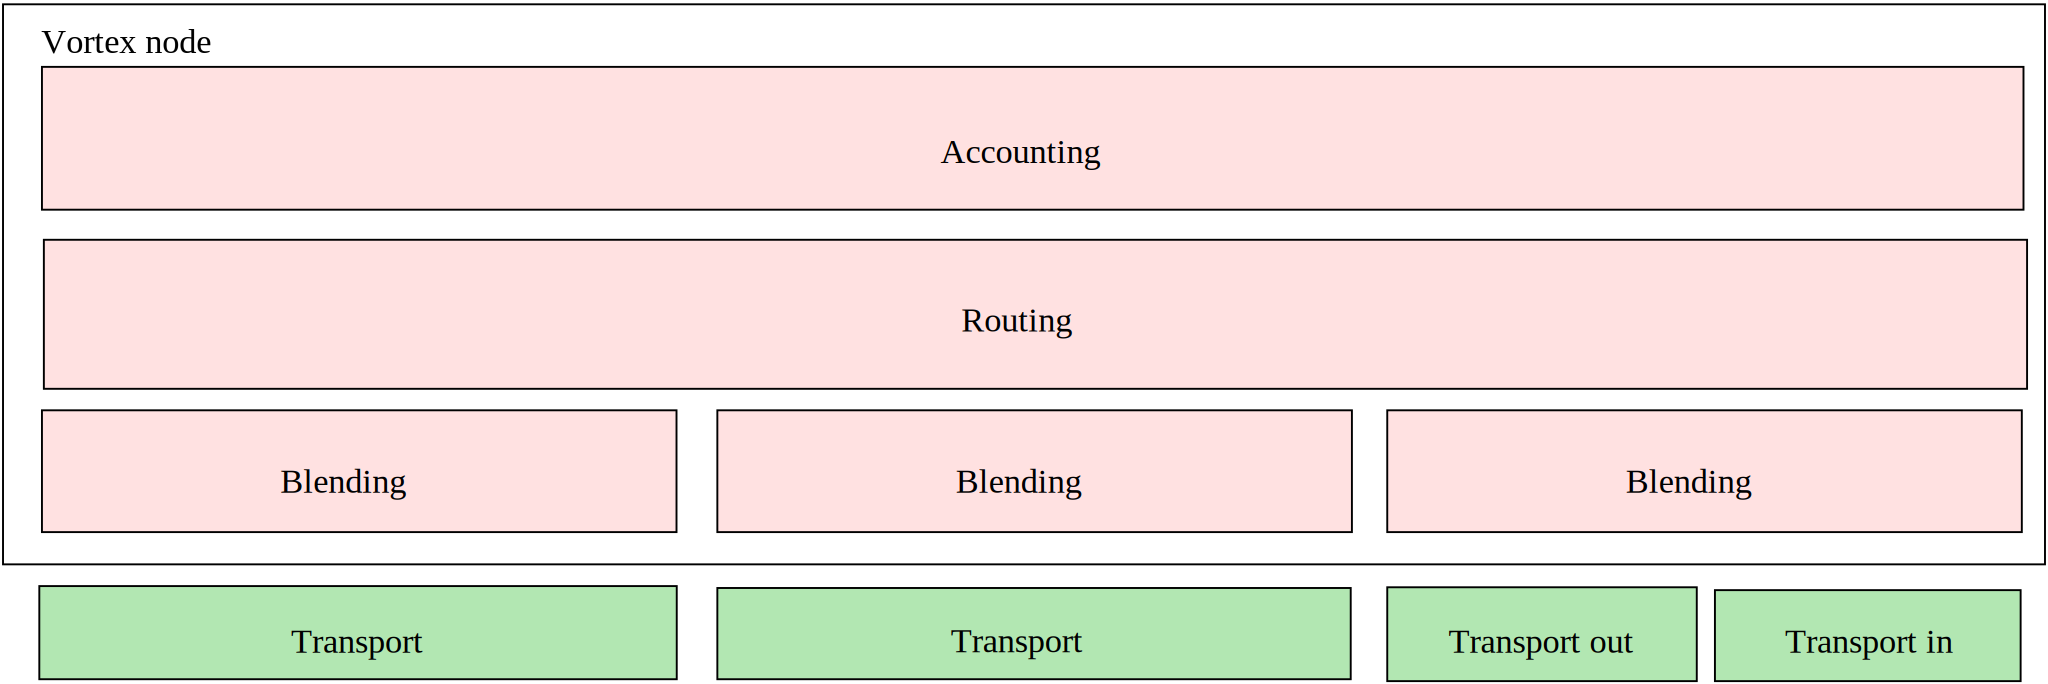
\includegraphics[width=\textwidth]{inc/layerDesign}
	\caption{The protocol layers}
	\label{fig:protocolLayers}
\end{figure}

The protocol is a four-layer protocol, as shown in figure~\ref{fig:protocolLayers}. We communicate with standard protocols, which we refer to as the transport layer. While included in the message flow, they do not form a part of the \VortexNode. The \VortexNode{} itself consists out of the three layers ``Blending'', ``Routing'', and ``Accounting''.

The blending layer is the bridging part linking a transport layer to the \VortexNode{}. It injects and extracts messages from the transport layer and passes the extracted messages to the routing layer. It may be either used as a protocol bridge (e.g., in the case of XMPP) or act as a sophisticated router (e.g., in the case of the email protocols, where mails are fetched or received on push event via POP3 or IMAP while sending messages using SMTP).

The routing layer receives unified standard messages from the blending layer processes them, possibly extracts messages for local delivery, and passes subsequently created messages to the blending layer.

This design is definitely implementable on a consumer device. On the other hand, it is scalable and suitable for a clustered environment. Blending can be done in a stateless manner, is even suitable for serverless computing, and thus largely scalable. Routing may be implemented either with horizontal partitioning along with a set of \defref{eID}s or on a serverless base with a unified storage in the background. The accounting layer acts as a controller and may be implemented as well as stateless service with a minimal NOSQL-storage for all \defref{eID}s. 

\chapter{Protocol}\label{sec:protocol}
\MessageVortex{} is a protocol piggybacking standard transport protocols somehow similar to S/MIME\cite{rfc2015} or PGP\cite{PGP}. Unlike these protocols, we need the capability to keep the presence of our messages secret.  The message itself should only be visible to an intended node.\MessageVortex{} itself is agnostic to the transport, but we do require appropriate blending to hide within the transport protocol. The information processed on a node and its associated meta-information should not leak any information about the processed message. 

Our system sends so-called \VortexMessages. These messages are hidden within a transport protocol (e.g., SMTP or XMPP) with a blending mechanism (e.g., the steganographic algorithm F5) and extracted by a blending layer. The extracted \VortexMessage{} is handed over to a routing layer. The \VortexMessage{} itself contains a header block, a routing block, and possibly some payload blocks. The header block contains all the information required to protect the system. The routing block contains instructions (so-called ``\defref{operation}s'') how the payload blocks have to be processed and where to send the resulting blocks. Those \defref{operation}s are one of the keys as information leaking happens in this step in most of the systems. We, therefore, crafted all \defref{operation}s very carefully to keep as much information secret as we could. These \defref{operation}s are the key to the system as they allow us to increase and decrease the size of a message without leaking what part of the data is a decoy and what not.

A payload may either be kept by the system for later processing with other messages, processed (possibly with different) payload blocks, or displayed to the "local user" as a message.

The general idea of the protocol is to form a network from nodes that mix and route messages between the sender and receiver. A routing block builder (\defref{RBB}), which is typically identical to the sender, has full control over almost all attributes of the message, and nodes are unable to learn anything from the message while routing. Each user has a node, and there may be additional nodes (public routing nodes) without a user connected to it. 

The message is either onion-like encrypted, split into parts and remerged, or blown up with redundancy information. 

This behavior results in a mixing like a system with a decoy generation in which even decoy generating nodes are unable to differentiate between real traffic and decoy as all blocks always contain parts of the message. Routing decisions are controlled by the builder of the routing block, and redundancy is possible and controlled by the routing block builder to make the system more stable.

In the following sections, we describe this protocol in detail. First, we build a terminology implicitly used in the previous chapters. Then we describe the key concepts and techniques of the protocol without in-depth analysis or reasoning. Implementation and operational aspects are discussed in part~\ref{sec:implementation} and part~\ref{sec:operation}. 


\section{Protocol Terminology}
For our protocol, we use the following terms:
\begin{itemize}
	\item \textbf{\defref{Sender}:} The user or process originally composing the message.
	\item \textbf{\defref{Recipient}:} The user or process destined to receive the message in the end.
	\item \textbf{\defref{User}:} Any entity, running a \MessageVortex{} node.
	\item \textbf{\defref{Router}:} Any node which is processing the message. Please note that all \VortexNode{}s are routers. This includes the senders' and recipients' node.
	\item \textbf{\defref{Message}:} The "real content" to be transferred from the sender to the recipient.    
	\item \textbf{\defref{VortexMessage}:} The encoded message passed from one node to another one. The \VortexMessage{} is considered before any embedding takes place. If embedded, we refer to such a message as "embedded \VortexMessage".
	\item \textbf{\defref{Payload}:} Any data transported in a \VortexMessage{} between routers with exception to the routing and header block, regardless of the meaningfulness or relevance to the \VortexMessage.
	\item \textbf{\defref{Decoy traffic}:} Any payload transported between routers that have no relevance to the message at the final destination.
	\item \textbf{\defref{Identity}:} A tuple of a routable address and a public key. This tuple is a long-living tuple but may be exchanged from time to time. An Identity is always assigned to a node, but one node may have multiple identities. 
	\item \textbf{\defref{eID}:} An identity created on any node with a limited lifetime anyone possessing the private key (proven by encrypting with it) is accepted as representative of that identity.
	\item \textbf{Routing Block Builder (\defref{RBB}):} An entity, which is building a routing block. Typically identical to either sender or recipient.
\end{itemize}

\section{Key Components}
The following sections list some of the key components of the system. Their understanding is essential for the understanding of the protocol as a whole. 

We first describe a single node and its identity. This node is always equivalent to a potential recipient. 

We then introduce the concept of \defref{workspace}s and ephemeral identities. These concepts are essential for the routing and accounting layers. They dictate memory and storage requirements and lay a foundation for the routing layer.

A node always consists of three layers and one or more transports connected to it. The understanding of their inner workings is essential to the understanding of the project as a whole. We emphasize on their main function and their inner workings without going into implementation details. These details are further discussed in part~\ref{sec:implementation}. We mainly focus on the data and the high-level processing done within these layers.

\subsection{Nodes and their identities}
We refer to a \VortexNode{} (node) as a system run by an individual containing a processing software processing \VortexMessages. Each node is connected to a transport layer protocol service (e.g., an IMAPv4 server as an endpoint for email or an XMPP server). 

Each node $o$ has at least one identity reflected by an asymmetric key pair $K_{host_o}$. Any node $p$ communicating with node $o$ must have the public key  $K^1_{host_o}$ of the node.

A node requires the key $K^1_{host_o}$ to encrypt a message for node $o$. This key know-how enables environments with censoring adversaries to withstand probing attacks, as, without the knowledge of such keys, no reply from a node is received. The transport endpoint itself is not secret. The usage as \VortexNode, however, is kept secret as long as the key is not known.

The protocol itself has the possibility to answer clear-text requests. So-called ``public nodes'' (see \ref{sec:vortexNodeTypes}) make use of such messages. They are, however, an exception. In general, all \VortexMessages{} are encrypted.

\subsection{Workspaces and Ephemeral Identities}
We dumped the approach for a system global unified storage for all message processing as such a design would allow an adversary to flood our storage. Instead, we introduced temporary storages suitable for a set of transaction belonging to a single identity or limited set of entities which collaborate. In our system, every transaction on a nose is assigned to an ephemeral identity (\defref{eID}). An \defref{eID} has a limited lifetime and is represented by an asymmetric key pair and has to be created on each \VortexNode{} taking part in a message processing. Each \defref{eID} has a storage assigned to which we refer as ``\defref{workspace}''.

An \defref{eID} is unique on every host and created on each \VortexNode{} by the routing block builder (\defref{RBB}). To create an \defref{eID}, an \defref{RBB} first sends a message with only a header block to the respective \VortexNode. The request contains the new identity, a reply block, and a request to create a new identity. The receiving \VortexNode will then typically sends a challenge back. A challenge may be the start of a hash bit sequence (also referred to as "puzzle"). The requester has then to resend the request with a header block. The requester must insert additional data in such a way that the start hash in its binary form matches the bit sequence provided. Another possibility is to request a payment in cryptocurrency. This allows us to commercialize routers in some countries where the usage of such routers is generally allowed.

The length of the requested bit sequence is chosen by the accounting layer at its own will. If the request is not answered in a given time, the \defref{eID} will be discarded. Analogous to an SYN-Flood attack, an adversary may try to overwhelm a \VortexNode{} with \defref{eID} creation requests. Such flooding will be much more costly for the adversary than for the \VortexNode{}, and such a node may decide to temporarily no longer accept new \defref{eID} requests without affecting already existing \defref{eID}s.

Each \defref{eID} has a lifetime, a maximum number of messages to be processed, and a maximum number of bytes to be sent assigned to it. The lifetime of an \defref{eID} is typically days and maybe up to a low number of months. Lifetimes may not be extended and are defined by the sender of the request. A node may accept or decline the request if the lifetime of the request or the state of the node does not meet its expectation. The puzzle sent in return may be a fixed value or related to the nodes' current state and load.

This system guarantees that a sender must invest considerable work (in terms of CPU time required) prior to using resources of a \VortexNode. A \VortexNode{} may raise the complexity of its puzzles when having a  high load. This allows for a single user to still obtain an \defref{eID} while increasing costs for an attacker considerably. Even if someone floods a node with new \defref{eID}s, already created \defref{eID}s are not affected as their \defref{workspace} has already been allocated.

The \defref{workspace} itself contains chunks of the messages (payload blocks) mapped to \defref{ID}s and \defref{operation}s. The \defref{operation}s transform one or more source \defref{ID}s onto one or more target \defref{ID}s. Any of these payload blocks may be assigned to a subsequent message as payload block by a routing block. An \defref{operation} or a payload block share the lifetime of the respective message header. If \defref{operation}s overlap in output blocks the newest \defref{operation} (arrived latest) wins. Arriving \VortexMessages{} map their payloads onto \defref{ID}s of the respective \defref{workspace} of the \defref{eID}. to allow such mapping the first IDs are special \defref{ID}s either mapping to the \defref{ID} 0 (message for local delivery) or \defref{ID}s 1-127 (always reflect the current message [ingoing or outgoing]).

This concept has certain downsides related to the expiry of \defref{eID}s. We will address them in section\ref{sec:newEID} and section~\ref{sec:replaceMURB}.

\subsection{Protocol Layers}
As already introduced in \ref{sec:reqSummary}, the protocol is built on multiple software layers. On the logic side, the protocol is split into two parts:
\begin{enumerate}
	\item Transport Layer\\
	Standard Internet infrastructures provide this layer. The primary goal is to hide or blend our protocol into regular traffic within that layer. Typical examples for such layers are SMTP or XMPP servers.
	\item Blending and subsequent layers (the Vortex infrastructure)\\
	Any user of the Internet may provide these layers. Since these layers may be only Vortex routing nodes or valid endpoints, the nodes may or may not be publicly known. In a first implementation, we build this system as a standard Java application. The primary goal is to compile it to native code afterward and run it on an SoC like infrastructure such as a RaspberryPi or port it to an android device.
	
	We may further split the Vortex infrastructure layers into
	\begin{enumerate}
		\item dBlending layer\\
		This layer receives messages from the Vortex system and creates transport layer conformant messages and vice-versa. In an ideal case, the messages generated by this layer are indistinguishable from any regular message traffic of the transport layer, and the embedded message is only detectable by the receiving node.
		\item Routing layer\\
		The routing layer disassembles and reassembles messages. 
		\item Accounting layer\\
		The accounting layer has three jobs. First, he has to authorize the message processing after the decryption of the header block by the blending layer. Secondly, he handles all header request blocks and the reply blocks. And third, it keeps track of the accounting regarding the sent messages. Its main purpose is to protect the system from misuse or flooding.    
	\end{enumerate}
\end{enumerate}

In total, we have four layers. The bottom-most layer consists of unmodified standard infrastructure for transport within the Internet, and the three layers on top build a single \VortexNode.

\subsection{Transport Layer}
The transport layer is a standard protocol within the Internet. It is neither a \MessageVortex{}-specific infrastructure, nor has it been modified for the purpose. Instead, it serves the purpose as a store and forward medium. This medium solves two major problems. First, no NAT traversal technology such as "TCP hairpins" or "hole punching" is required. And secondly, it compensates for short outages due to regional routing problems to the end-user.

A transport layer should have some generic properties:
\begin{itemize}
	\item Widely adopted 
	\item Reliable
	\item Symmetrical built 
\end{itemize}

For a more detailed description of the criteria, see section~\ref{sec:transportCriteria}.

For our first tests, we used a custom transport layer, allowing us to monitor all traffic quickly, and build structures in a very flexible way. This transport layer works locally or in a broadcast-based network with a minimum amount of work for setup and deployment. The API we used may, however, be used to support almost any kind of transport protocol.

In section~\ref{sec:transportProtocols}, we make a short analysis going through some common protocols outlining the strength and weaknesses of common transport protocols within the Internet.

After that, we focussed on the protocols identified in the previous sections for transport:
\begin{itemize}
	\item \defref{SMTP}
	\item \defref{XMPP}
\end{itemize}
For the prototype, we have implemented an SMTP transport agent and the respective blending layer.

\subsubsection{Blending Layer\label{sec:blendingLayer}}
The blending layer is taking care of multiple problems:
\begin{itemize}
	\item It is translating the message block into a suitable format for transport\\
	This translation includes jobs such as embedding a block as encoded text, as a binary attachment or hide it within a message using steganography. Another demanding task in this context is to create credible content for the transport message itself.
	\item Extract incoming blocks\\
	Identify incoming messages containing a possible block and extract it from the message.
	\item Do housekeeping on the storage layer of the transport protocol\\
	Access protocols such as POP and IMAP require that messages are deleted from time to time to stay below the sizing quotas of an account. To manage this transport layer account is the job of the blending layer.
\end{itemize}

There is no specification on the housekeeping part of the blending layer, as this part is specific to the requirements of the account owner. We do, however, recommend to handle messages precisely as if the messages would be handled on an account handled by a human. This means that some messages. 

The blending is currently done by merging the \VortexMessage using either F5 as described in \cite{f5} or by doing plain blending, which is a binary embedding. This means that we require jpeg images included in the SMTP message. 

\paragraph{Processing of a Message received from the Transport Layer}~\\
We define the blending layer to work as follows when receiving messages:
\begin{enumerate}
	\item Log arrival time on the transport layer.
	\item Extract possible \VortexMessage.
	\item Apply decryption on a suspected header block of \VortexMessage.
	\item Identify the header block as valid by querying the accounting layer.
	\item Extract and decrypt subsequent blocks.
	\item Pass extracted blocks and information to the routing layer.
\end{enumerate}

\paragraph{Processing of a Message received from the Routing Layer}~\\
We define the blending layer to work as follows for sending messages:
\begin{enumerate}
	\item Assemble message as passed on by the routing layer.
	\item Using the blending method specified in the routing block, build an empty message. 
	\item Create a message decoy content.
	\item Send the message to the appropriate recipient using the transport layer protocol.
\end{enumerate}

\paragraph{Credible Content Creation for the Transport Layer}~\\
One of the most demanding tasks of the blending layer is to create transport protocol messages. In \cite{oakland2013-parrot}, \citeauthor{oakland2013-parrot} expresses that it is easy for a human to determine decoy traffic as the content is easily identifiable as generated content. While this is up to all that we know true, there is a possibility here to generate "human-like" data traffic to a certain extent. For the blending layer, it is not necessarily required to mimic human messages. Instead, the blending layer may generate messages such as password recovery messages, monitoring messages, and even \defref{UBE}-like content. All these messages have required properties in common. First, all of them are machine-generated messages which are modified quite often. All of these messages are known to be sent and possibly adapted individually. 

For the blending itself, we required a steganographic algorithm. After reviewing the options, we decided to go for F5\cite{f5} as a steganographic algorithm. It is a reasonably well-researched algorithm, which attracted many researchers. The original F5 implementation had a detectable issue with artifacts\cite{F5broken} caused by the recompression of the image. This issue was caused only due to a problem in the reference implementation, and the researchers have provided a corrected reference implementation without the weakness.

We looked for other steganographic algorithms, but were unable to find any other suitable algorithm apart from F5, which fulfilled the following set of criteria:
\begin{itemize}
	\item Unbroken.
	\item Researched.
	\item Suitable for embedding in lossy compressed, common image formats (e.g., jpeg).
	\item An implementation or a well-specified algorithm exists.
\end{itemize}

We decided to keep our plain embedding algorithm in the implementation. It already requires an in-depth analysis or a human to detect embedding, and the message itself is, even if detected, well-protected. Its biggest most strength is, however, its efficiency. This algorithm is, however, only suitable for public nodes matching up to an observing adversary (as defined in section~\ref{sec:adversary}). It must not be used in environments where a censoring adversary is suspected.

When using F5, jpeg images are required. Imagery requires to be at least eight times the size of the message embedded. Unlike other approaches harvesting random pics or obtaining them from a local repository, we recommend using machine-generated images such as rendered content. We recognize that custom Gravatars, router and usage graphs of services, or render services are suitable imagery material for our purpose. The message content would obviously be machine-generated content and not being suspect. This would effectively render the dead parrot problem as described in \cite{oakland2013-parrot} ineffective. 

\subsubsection{Routing Layer\label{sec:routingLayer}}
A routing layer needs to receive all payload and routing blocks, and process them (For an exact outline of the routing block, see section~\ref{sec:vortexMessage}). These blocks are stored in a suitable list within the \defref{workspace} of the \defref{eID} identified by the header block.

Within the routing block, we find a set of instructions, next \VortexNodes information, and the encrypted routing blocks for the messages to be assembled. A simplified representation of a routing block is shown in figure~\ref{fig:mathRoutingSimplified}.

\begin{figure}[!ht]
	\begin{align}
	\mathbf{ROUTING_o}           = & \langle [ \mathbf{ROUTINGCOMBO} ] *, \mathbf{replyBlock},mapping* \rangle\\  
	\mathbf{ROUTINGCOMBO}        = & \langle processIntervall, K_{peerN+1}, recipient, \mathbf{nextMP}, \mathbf{nextHP}, \nonumber \\
	& \mathbf{nextHEADER}, \mathbf{nextROUTING}, \mathbf{assemblyInstructions} \rangle\\
	\mathbf{PL}                  = & \langle \text{payload octets} \rangle *\\ 
	\mathbf{nextMP}              = & E^{K^1_{host_{o+1}}} \left( K_{peer_{o+1}} \right)\\
	\mathbf{nextHP}              = & E^{K^1_{host_{o+1}}} \left( K_{sender_{o+1}} \right)\\
	\mathbf{nextHEADER}          = & E^{K_{sender_o}} \left( \mathbf{HEADER_{o+1}} \right)\\
	\mathbf{nextROUTING}         = & E^{K_{sender_o}} \left( \mathbf{ROUTING_{o+1}} \right)\\    
	\mathbf{operations}          = & \langle \text{list of operations} \rangle \\
	\mathbf{assembyInstructions} = & \langle  blendingInformation, nextHop, \langle \text{mapping operation} +\rangle \rangle
	\end{align}
	\caption{Simplified representation of a routing block}
	\label{fig:mathRoutingSimplified}
\end{figure}

The routing of a message is simple. A \defref{workspace} of an \defref{eID} contains routing blocks and payload blocks. A routing block has an active time window defined in the header block. Anytime during that time window, a routing layer processes the routing instructions contained in the assembly operations of the routing block. If successful, the message will be sent using the specified blending layer and target address.

The routing layer stores the main information assigned to the operation of routing messages. The following data has to be kept for routing within the \defref{eID}s \defref{workspace}:
\begin{itemize}
	\item $\mathbf{Build[]}\langle expiry, buildOperation \rangle$\\
	The array $\mathbf{Build[]}$ is a list of building instructions for a message. The server may decide at any time to reject a too big list or long-living message. Thus, he may control the size of this list as well. However, controlling the size of this list will most likely result in the non-delivery of a message. 
	
	The $buildOperation$ is extracted by enumerating $operation*$ while $expiry$ is the upper bound of the $processIntervall$.
	\item $\mathbf{Payload[]}\langle expiry, payload, id \rangle$\\
	The array $Payload[]$ reflects a list of all currently active payloads. Servers may decide to store derivatives of payloads. However, as derived payloads inherit their expiry from the generating operation, such behavior may be safely omitted and operations executed if their result is required.
	
	\item $\splitatcommas{\mathbf{Route[]}\langle processIntervall, blendingInformation, nextHop, \mathbf{nextMP}, \mathbf {nextHP}, \mathbf{nextHeader}, \mathbf{nextRouting}, K_{peer_{o+1}}, \mathbf{assemblyInstructions} \rangle}$\\
	The list of routing information triggers processing. At a randomly chosen time defined in the $processIntervall$, a message is composed. The message is assembled by doing $\splitatcommas{\langle \mathbf{nextMP}, E_{K_{peer_{o+1}}}\langle \mathbf{nextHP}, \mathbf{nextHEADER}, \mathbf{nextROUTING}, payload* \rangle \rangle}$. The payloads are created with the help of the arrays $build[]$ and $payload[]$, and as soon as the message is authorized by accounting and passed to the blending layer, the entry in this list is discarded.
\end{itemize}

\subsubsection{Accounting Layer\label{sec:accountingLayer}}
The accounting layer keeps tracks of all information required assigned to ephemeral identities (\defref{eID}). It is queried by the blending Layer and routing Layer for authorization of the operations. The accounting layer manages the following tuples of information:

% List duplicated in Accounting layer in implementation and protocol
\begin{itemize}
	\item $\mathbf{eID[]}\langle expiry, pubKey, mesgsLeft, bytesLeft \rangle$\\
	The $\mathbf{eID}$ tuple is the longest living tuple. It reflects an ephemeral identity and exists as long as the current identity is valid. All other tuples are short living lists. As the server decides if he accepts new identities or not, the size of this data is controllable. 
	\item $\mathbf{Puzz[]}\langle expiry, request, puzzle \rangle$\\
	The array $\mathbf{Puzz[]}$ is a list of not yet solved puzzles of this \defref{eID}. Every puzzle has a relatively short lifespan (typically below 1d). A routing node controls the size of this list by only accepting requests to a certain extent. Typically this list should not surpass two entries as we should have either a maximum of two quota requests or one identity creation request open.
	\item $\mathbf{Replay[]}\langle expiry, serial, numberOfRemainingUsages \rangle$\\
	The array $\mathbf{Replay[]}$ is a list of serials. List entries are created upon their first usage and remain active until the block is expired. 
\end{itemize}


\subsection{VortexMessages}\label{sec:vortexMessage}\index{VortexMessage}
A \VortexMessage{} is built by combining multiple loosely interconnected blocks. We first name the blocks and their function, and then we explain the inner working of the blocks and do some reasoning why the block has been built as it is. 

Figure~\ref{fig:messageOutline} shows an outline of the block structure of a message destined to $host_o$. For a mathematical representation, see figure~\ref{fig:mathMessage}.

\begin{figure}[ht]
	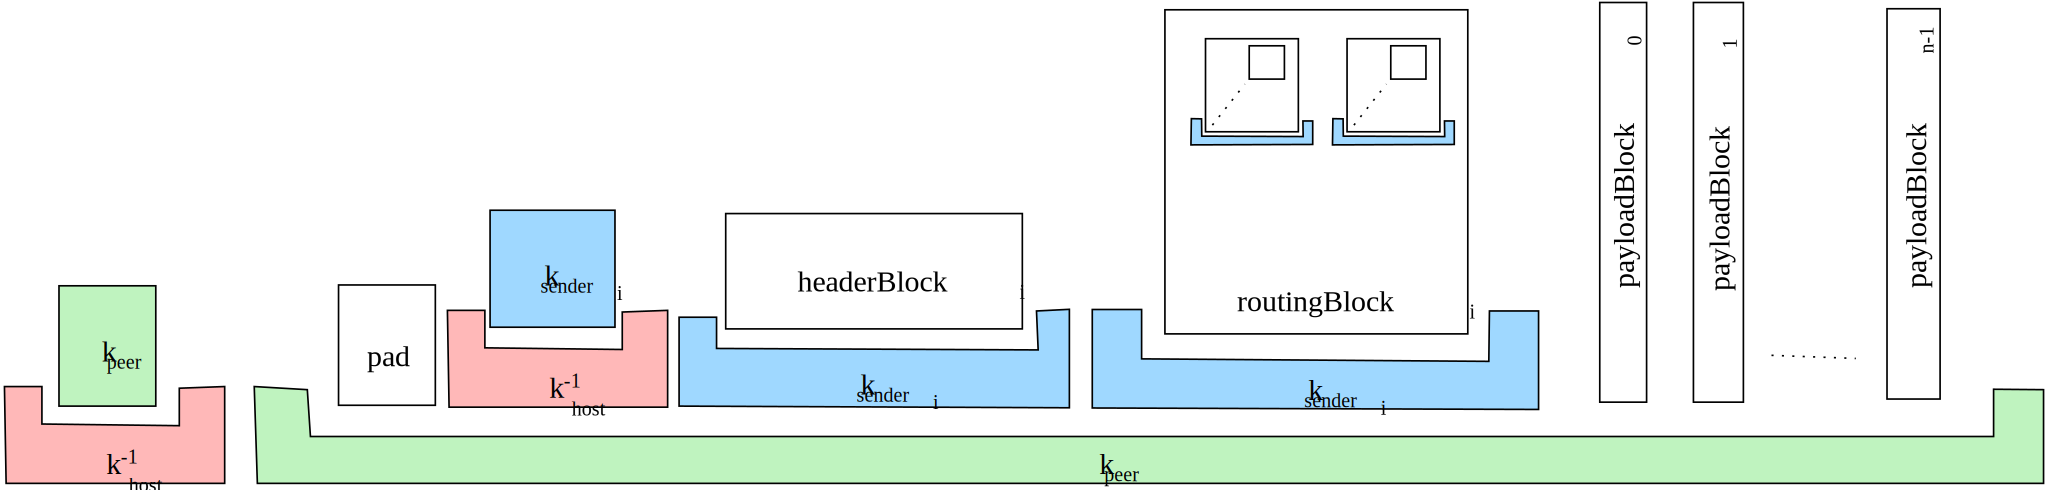
\includegraphics[width=\textwidth]{inc/blockLayoutSimplified}
	$\splitatcommas{\langle \mathbf{MPREFIX_o}, E_{K_{peer_{o+1}}}\left( \mathbf{HPREFIX_o}, \mathbf{HEADER_o}^{K_{sender_o}}, \mathbf{ROUTING_o}^{K_{sender_o}}, payload* \right) \rangle}$
	\caption{Simplified message outline visually and in math}
	\label{fig:messageOutline}
\end{figure}

The first block is the message prefix block $\mathbf{MPREFIX_o}$, which has been encrypted with the public key of the receiving node $K^1_{host_o}$. This block contains the key for decrypting the whole rest of the message. Each PREFIX block contains a symmetrical ey and the specification on how to encrypt or decrypt with it (mode, padding, IV, and other possibly required parameters) in ASN.1 encoding. 

Immediately following the message prefix block, we have the inner message block. This message blocks contain three more blocks and a variable number of payload blocks. The inner message is encrypted with the symmetrical peer key $K_{peer_o}$. This peer key is specific to this message and nowhere reused. It is only known by the two peer hosts $host_o$ and $host_{o-1}$, and the routing block builder (\defref{RBB}). More importantly, $host_{o-1}$ does not need to know the host key of $host_o$. Therefore, relaying a message to $host_o$ does not enable $host_{o-1}$ to communicate with $host_o$. 

The blocks $HEADER_o$ and $ROUTING_o$ are protected with an additional key $K_{sender_o}$. The decryption key is obtained by $host_o$ from the header prefix block $\mathbf{HPREFIX}$. After only decrypting the header block $\mathbf{HEADER}$ and verifying its signature, the accounting layer may check if further processing is authorized. The splitting of the two keys allows us to\ldots
\begin{itemize}
	\item \ldots send a message to $host_o$ without $host_{o-1}$ knowing the host key of $host_o$.
	\item \ldots hide the structure of the message itself.
	\item \ldots keep the content of $\mathbf{HEADER_o}$, and $\mathbf{ROUTING_o}$ secret from $host_{o-1}$.
\end{itemize}

After authorization by the accounting layer, the header block is processed as outlined in section~\ref{sec:processingIncommingMessages}. Basically, we just add the routing blocks and payload to the respective \defref{workspace} and wait for the routing layer to process the information.

Looking at a full \VortexMessage, we get the protocol outline, as shown in \eqref{eq:vortexMessage} on page~\pageref{eq:vortexMessage}.

\begin{figure*}[!ht]
	\begin{align}
	\mathbf{VORTEXMESSAGE}       = &\langle \mathbf{MP}^{K^{-1}_{host_o}}, INNERMESSAGE \rangle \label{eq:vortexMessage} \\ 
	\mathbf{INNERMESSAGE}        = &\langle \mathbf{CP}^{K^{-1}_{host_o}}, \mathbf{H}^{K_{sender_o}}, E^{K^{-1}_{sender_o}}\left(H\left(\mathbf{HEADER}\right)\right), \left[\mathbf{R}^{K_{senderN}}\right], \left[\mathbf{PL}\right]*\rangle^{K_{peerN}} \label{eq:innerMessage}\\
	\mathbf{MP}^{K^{-1}_{hostN}} = &E^{K^{-1}_{hostN}}\left(\mathbf{PREFIX}\langle K_{peerN}\rangle \right)\\ 
	\mathbf{HP}^{K^{-1}_{hostN}} = &E^{K^{-1}_{hostN}}\left(\mathbf{HPREFIX}\langle K_{senderN}\rangle \right)\\ 
	\mathbf{H}^{K_{senderN}}     = &E^{K_{senderN}}\left(\mathbf{HEADER}\right)\\  
	\mathbf{HEADER}              = &\langle K^{1}_{senderN}, serial, maxReplays, validity, [requests, requestRoutingBlock],\nonumber\\ 
	& [puzzleIdentifier, proofOfWork] \rangle \\  
	\mathbf{R}^{K_{senderN}}     = & E^{K_{senderN}}\left(\mathbf{ROUTING}\right)\\ 
	\mathbf{ROUTING}             = & \langle [ \mathbf{ROUTINGCOMBO} ] *, forwardSecret, \mathbf{replyBlock},\mathbf{operations} \rangle\\  
	\mathbf{ROUTINGCOMBO}        = & \langle processIntervall, K_{peerN+1}, recipient, \mathbf{nextMP}, \mathbf{nextHP}, \nonumber \\
	& \mathbf{nextHEADER}, \mathbf{nextROUTING}, \mathbf{assemblyInstructions} \rangle\\
	\mathbf{nextMP}              = & E^{K^1_{host_{o+1}}} \left( K_{peer_{o+1}} \right)\\
	\mathbf{nextHP}              = & E^{K^1_{host_{o+1}}} \left( K_{sender_{o+1}} \right)\\
	\mathbf{nextHEADER}          = & E^{K_{sender_o}} \left( \mathbf{HEADER_{o+1}} \right)\\
	\mathbf{nextROUTING}         = & E^{K_{sender_o}} \left( \mathbf{ROUTING_{o+1}} \right)\\    
	\mathbf{operations}          = & \langle \text{list of operations} \rangle \\
	\mathbf{assembyInstructions} = & \langle  blendingInformation, nextHop, \langle \text{list of mapping operations}\rangle\rangle\\
	\mathbf{PL}                  = &\langle \text{payload octets} \rangle *\\ 
	\end{align}
	%\captionsetup{labelformat=empty}
	\caption{Detailed representation of a VortexMessage}
	\label{fig:mathMessage}
\end{figure*}

The routing log block is an onionized block. It contains at least a $forwardSecret$, which must match up with the header blocks $forwardSecret$. This mechanism is required to guarantee that routing blocks are not exchanged. The $replyBlock$ provides a possibility, if provided, to contact the original sender of the message without knowing him. It is just a routing block with instructions on how to prepare the message to be sent. The routing combos contain all the necessary information and prebuilt blocks to create the subsequent messages.

At the very end, we got the payload. These blocks are simply added to the \defref{eID}s \defref{workspace}.

The double encryption of the routing and header block, are doubly encrypted. We could argue that the inner message block should not be encrypted with a peer key. This looks like a flaw at first sight but is, in fact, a feature that is very important. Without this key, any independent observer with knowledge about the blending capabilities of a receiving node may\ldots
\begin{itemize}
	\item Easier to identify the block structure.\\ 
	This statement remains regardless of whether ASN.1 or length prefixed structures are used. If the structure of a \VortexMessage is easily identified, the messages may be logged or dropped.
	\item Identify the routing block size.\\
	The value of this information is only minimal as it only reflects the complexity of the remaining routing information indirectly.
	\item Identify the number of payload blocks and their respective sizes. \\
	Sizing information is valuable when following the path of a message.
\end{itemize}

\subsubsection{Message Structure Related to Censorship Circumvention}
It is important to note that there is no structure dividing the encrypted peer key from the Inner message block. The size of the peer key block is defined by the key and algorithm of the host key. 

The whole \VortexMessage is, looking from outside, a structureless blob with a maximum of entropy caused by the encryption employed. 

This is intentional and by design. Plain embedding uses furthermore a method of splitting, which allows a message block to be embedded in chunks in carrier information. By design, neither the message nor their embedding display detectable attributes allowing them to identify the message. 

Exactly as with the routing operations, great care has been applied. Any random sequence of bytes may be interpreted as valid chunking. For more exact implementation details on chunking, see section~\ref{sec:chunkingPlain}.

\subsubsection{Message Structure Related to Information Leaking}
From the inside, the $\mathbf{INNERMESSAGE}$ (see \ref{eq:innerMessage}) is built as a structure leaking the absolute minimum of information. A node receiving and decoding the message will learn the following information:
\begin{itemize}
	\item IP of the sender of the transport layer.
	\item The address and embedding schemes of all receiving transport layers.
	\item The size of the payload blocks.
	\item The size of the subsequent routing blocks.
	\item The peer key $K_{peer_o}$.
	\item The size of the prefix blocks.
\end{itemize}

It is unable to extract the following information:
\begin{itemize}
	\item The required keys to communicate with the suspected peer node.
	\item Any information related to message size, content, or recipient.
\end{itemize}

\subsection{Routing Operations\label{sec:operations}}
The routing operations build the core as they define the capabilities of the mixing. We decided to introduce three different classes of operations. Wherever we employ crypto, operations, we may choose the operation required for the operation. No choices exist for the core Reed-Solomon-Function, the padding and spitting operation related to it, and the split and merge operations.

\subsubsection{$addRedundancy$ and $removeRedundancy$ Operations}
I this section we focus on the core operation of our system. The $addRedundancy$ and $removeRedundancy$ allow growing message sizes in our system without allowing to identify the decoy traffic. 

The Lagrange functions have been proposed in \cite{shamir1979share} and further more generalized in \cite{mceliece1981sharing} for sharing secrets. The general idea about all proposed schemes is to distribute informations and restrct access to it so that only if a specified number of shares are captured a secret may be rebulit. Unlike proposed in these papers we do not apply privacy to our protocol by sharing the data among many points. Instead we use lagrange functions to create decoy traffic. By doing so even a creator of traffic is unable to tell message traffic from decoy traffic apart. 

These operations build the core of the routing capabilities of a node. The operation allows an \defref{RBB} to add to a message redundancy information or to rebuild a block from a chosen set of information. 

The operation itself is shown in figure~\ref{fig:addRedundancyOperation}. 
\begin{figure}[ht]\centering
	\includegraphics[width=0.8\columnwidth]{inc/addRedundancyOp}
	\caption{Outline of the addRedundancy operation}
	\label{fig:addRedundancyOperation}
\end{figure}

It may be subdivided into the following operations:
\begin{itemize}
	\item Pad the original message block in such a way, that all resulting blocks are a multiple of the block size of the encrypting cipher.
	\item Apply a Reed Solomon operation in a given GF space with a vanderMonde matrix.
	\item Encrypt all resulting blocks with unpadded, symmetrical encryption.
\end{itemize}

The padding applied in the first step is non-standard padding. The reason for this lies in the properties required by the operation. The presence of standard padding may leak, whether the block has been successfully decrypted or not. Therefore, we created a padding with the following properties:
\begin{itemize}
	\item The padding must not leak whether the rebuild cycle of the operation was successful or not.
	\item Anyone knowing the routing block content and the transmitted message must be able to predict any treated block, including all padding bytes.
	\item The padded content must provide resulting blocks of required size to enable non-padded encryption after the RS operation
	\item The padding must work with any size of padding space.
	\item The padded and encrypted block must not leak an estimate of the original content.
\end{itemize}

The padded block $\mathbf{X}$ is created from a padding value $p$, the unpadded block $\mathbf{M}$ and a series of padding bytes. We build $\mathbf{X}$ for a function $RS_{\text{m of n}}$ (allows adding $m$ redundancy blocks) and an encryption block $\mathbf{M}$ sized $K$ as follows:
\begin{eqnarray}
i          & = & len(\mathbf{M})\\
e          & = & k \cdot n\\
l          & = & \left\lceil\frac{i + 4 + C2 }{e}\right\rceil\cdot e\\
p          & = & i + \left( C1 \cdot l \pmod{\left\lfloor\frac{2^{32}-i}{l}\right\rfloor\cdot l}\right)\\
\mathbf{X} & = & \langle p,\mathbf{M},R_{t}\left(s,l-i-4\right)\rangle
\end{eqnarray}    
The remainder of the input block, up to length $l$, is padded with random data. The random padding data may be specified by RBB though a PRNG spec $t$ and an initial seed value $s$. The message is padded up to size $L$. All resulting, encrypted blocks do not require any padding. This because the initial padding guarantees that all resulting blocks are dividable by the block size of the encrypting function. If not provided by an RBB, an additional parameter $C1$ is chosen as random positive integer and $C2=0$  by the node executing the operation.

To reverse a successful message recovery information of a padded block $\mathbf{X}$, we calculate the original message size by extracting $p$ and doing $len(\mathbf{M})=p \pmod{ len(\mathbf{X})}$.

This padding has many important advantages:
\begin{enumerate}
	\item The padding does not leak if the rebuilding of the original message was successful. Any value in the padding may reflect a valid value.
	\item Since we have a value $C2$, the statement that a message size is within $len(\mathbf{X})<size<(len(\mathbf{X})-k\cdot n)$ is no longer true and any value smaller $len(\mathbf{X})-k\cdot n$ may be correct as well.
	\item An RBB may predict the exact binary image of the padded message when specifying $C1$, $C2$, and $R_{t}(s,)$.
	\item A node knowing the original parameters $C1$, $C2$, and the initial PRNG seed $s$ can detect successful decryption.
\end{enumerate}

Apart from being non-standard padding, the padding has additional downsides:
\begin{itemize}
	\item The padding is inefficient compared to simple paddings such as PKCS\#7
	\item The padding requires an initialized PRNG to generate the padding.
	\item Depending on the chosen parameters, the padding overhead may become significant. 
\end{itemize}

After the padding, the date is ready for the Reed-Solomon part of the operation. We first group the data vector into a matrix $\mathbf{A}$ with $m$ columns to do the operations efficiently. The previous padding guarantees that all columns have a length, which is dividable by the block size of the encryption step applied later.

\begin{eqnarray}
t          & = & n-1\\in bytes
\mathbf{A} & = & vec2mat\left(\mathbf{X},\frac{len\left(\mathbf{X}\right)}{m}\right)\\
\mathbf{V} & = & \left(\begin{matrix}
0^0 & 0^1 & 0^2 & \cdots & 0^{(m-1)} \\
1^0 & 1^1 & 1^2 & \cdots & 1^{(m-1)} \\
2^0 & 2^1 & 2^2 & \cdots & 2^{(m-1)} \\
\vdots & \vdots & \vdots & \ddots & \vdots \\
t^0 & t^1 & t^2 & \cdots & t^{(m-1)}
\end{matrix}\right)\\
\mathbf{P} & = & \mathbf{V}\mathbf{A} \left(GF\left(2^\omega\right)\right)\\
\langle \mathbf{Q_1}, \ldots , \mathbf{Q_n} \rangle & = & row2vec(P)\\
R_i & = & E^{K_i}\left(Q_i\right)
\end{eqnarray}    

We apply the Reed-Solomon function by employing a Vandermonde matrix ($\mathbf{V}$). We build the data matrix ($\mathbf{A}$) by distributing the data into $\frac{len\left(\mathbf{X}\right)}{m}$ columns. This results in a matrix with $m$ rows. Unlike in error-correcting systems, we do not normalize the matrix so that the result of the first blocks is equivalent to the original message. Instead, the error-correcting information is distributed over all resulting blocks ($\mathbf{Q_i}$). Since the entropy of the resulting blocks is lowered as shown in figure~\ref{fig:entropy} and may thus leak an estimate of how a resulting block may have been treated, we added the encryption step to equalize entropy again. The previously introduced padding guarantees that there is no further padding on block-level required. The key used to encrypt the single blocks must not be equivalent. Equivalent keys have the side effect encrypting equal blocks into the same cyphertext. We observed faint but statistically relevant reminders of the unencrypted graphs when treating the same block with the same key and different redundancy parameters.

\subsubsection{$encrypt$ and $decrypt$ Operations}
The encrypt and decrypt operations are essential for the requirement that tagging should not be possible. Unlike the $addRedundancy$ and $removeRedundancy$, the splitting operations do not feature any encryption step after splitting or merging. Reusing a payload block that has only been split or merged would repeat the payload pattern on multiple nodes during transfer. That is why we require to have encryption.

The reason for not building this step into the split and merge function was simple. We needed a separate encryption step to be able to work as an onionizing system, and there were use cases where integrated encryption did not make sense. For further details on this topic, see section~\ref{sec:routingStrategies}.


\subsubsection{$mergePayload$ and $splitPayload$ operation}
The $splitPayload$ operation splits a payload block into two chunks of different or equal sizes. The parameters for this operation are:

\begin{itemize}
	\item source payload block $pb_1$
	\item fraction $f$\\
	A floating-point number which is describing the size of the first chunk. If the fraction is "1.0", then the whole payload is transferred to the second target chunk
\end{itemize}

If $len(pb_1)$ expresses the size of a payloadblock called $pb_1$ in bytes, then the two resulting blocks of the SpitPayload Operation $pb_2$ and $pb_3$ have to follow the following rules:

\begin{eqnarray}
split(f, pb_1) & = &\langle pb_1, pb_2 \rangle\\
pb_1.startsWith(pb_2)\\
pb_1.endsWith(pb_3)\\
len(pb_2) & = & floor(len(pb_1)\cdot f)\\
len(pb_1) & = & len(pb_2) + len(pb_3)
\end{eqnarray}

The $mergePayload$ operation combines two payload blocks into one. The parameters for this operation are:

\begin{itemize}
	\item first source payload block $pb_1$
	\item second source payload block $pb_2$
\end{itemize}

If $len(pb)$ expresses the size of a payloadblock called $pb$ in bytes then resulting block of the MergePayload Operation $pb_3$ have to follow the following rules:

\begin{eqnarray}
merge(pb_1, pb_2) & = & pb_3 \\
pb_3.startsWith(pb_1)\\
pb_3.endsWith(pb_2)\\
len(pb_3) & = & len(pb_1) + len(pb_2)
\end{eqnarray}

Unlike other operations, this operation has no encryption step attached to it. We usually attached an encryption step to remove repeating patterns from the \VortexMessage stream.

It has to be mentioned that this operation tuple has some issues when it comes to floating-point implementations. They are solvable but had to be specified unexpectedly precisely in order to enable a true cross-platform implementation. For more information regarding the issue and exact implementation, see section~\ref{sec:implOperations}.


\section{Summary}
The \MessageVortex{}-Protocol is split into the four layers ``Transport'' (a common internet standard protocol), ``blending'' (extracting and embedding \VortexMessages), ``Routing'' (A layer reassembling messages according to received instruction), and ``Accounting'' (Keeps track of all stored data and discards expired information).

All nodes are realized in decentral devices such as computers or mobile phones. Messages are hidden with either plain embedding or (referred) F5 in the transport layer message. The routing layer processes messages by applying operations to messages. Valid operations are encrypt or decrypt a message chunk, split a message chunk into two parts, merge two parts into one, or add or remove redundancy information. The last operation is the most valuable. This operation allows by employing an extended Reed-Solomon-Operation to add decoy traffic to the message flow without enabling a node to identify such traffic. Furthermore, it allows a sender to send parts of a message through multiple chains of routing nodes to a recipient. Each message itself does not leak the message content since depending on the completing block, any message with appropriate length may be valid.

The routing itself is done in a temporarily allocated storage called ``\defref{workspace}'', which is tied to an ephemeral identity (\defref{eID}) represented by an asymmetric key pair. To get an \defref{eID}, a sender typically solves a crypto puzzle. 

Payloads of \VortexMessages{} are mapped into the \defref{workspace}{} and are assigned a unique \defref{ID}{} within that workspace. The subsequent \defref{routing block}s and their \defref{operation}s are added as well and processed in a time interval defined by the \defref{RBB}.

